\documentclass{article}
\title{CS 205 Homework 6}
\author{Keith Lehman, kpl56@scarletmail.rutgers.edu}

\usepackage[margin=0.5in]{geometry}
\usepackage{graphicx}

\begin{document}
\maketitle

\begin{enumerate}

\item In a Boolean algebra, every element $x$ has an inverse element $\bar{x}$ such that $x + \bar{x} = 1$ and $x \bar{x} = 0$. Show that this inverse is unique. \\
    Proof by contradiction. Assume there are two values $y$ anad $z$ that are both inverses of $x$. From this, $x + y = x + z = 1$ and $xy = xz = 0$. From these statements, if x is removed, it can be seen that $y$ must equal $z$. 

\item The NAND logic gate is \textbf{universal}, meaning that using gate alone, we can implement any of the other logic gates. Find a way to derfine NOT, AND, and OR, using only NAND gates and the input variables $x$ and $y$. \\
\begin{enumerate}
\item NOT($x$) = NAND($x$, $x$) 
\item AND($x$, $y$) = NAND(NAND($x$, $y$), NAND($x$, $y$))
\item OR($x$, $y$) = NAND(NAND($x$, $y$), NAND($x$, $x$), NAND($y$, $y$))
\end{enumerate}

\item Using a Kanaugh map, find a minimal expression: \\
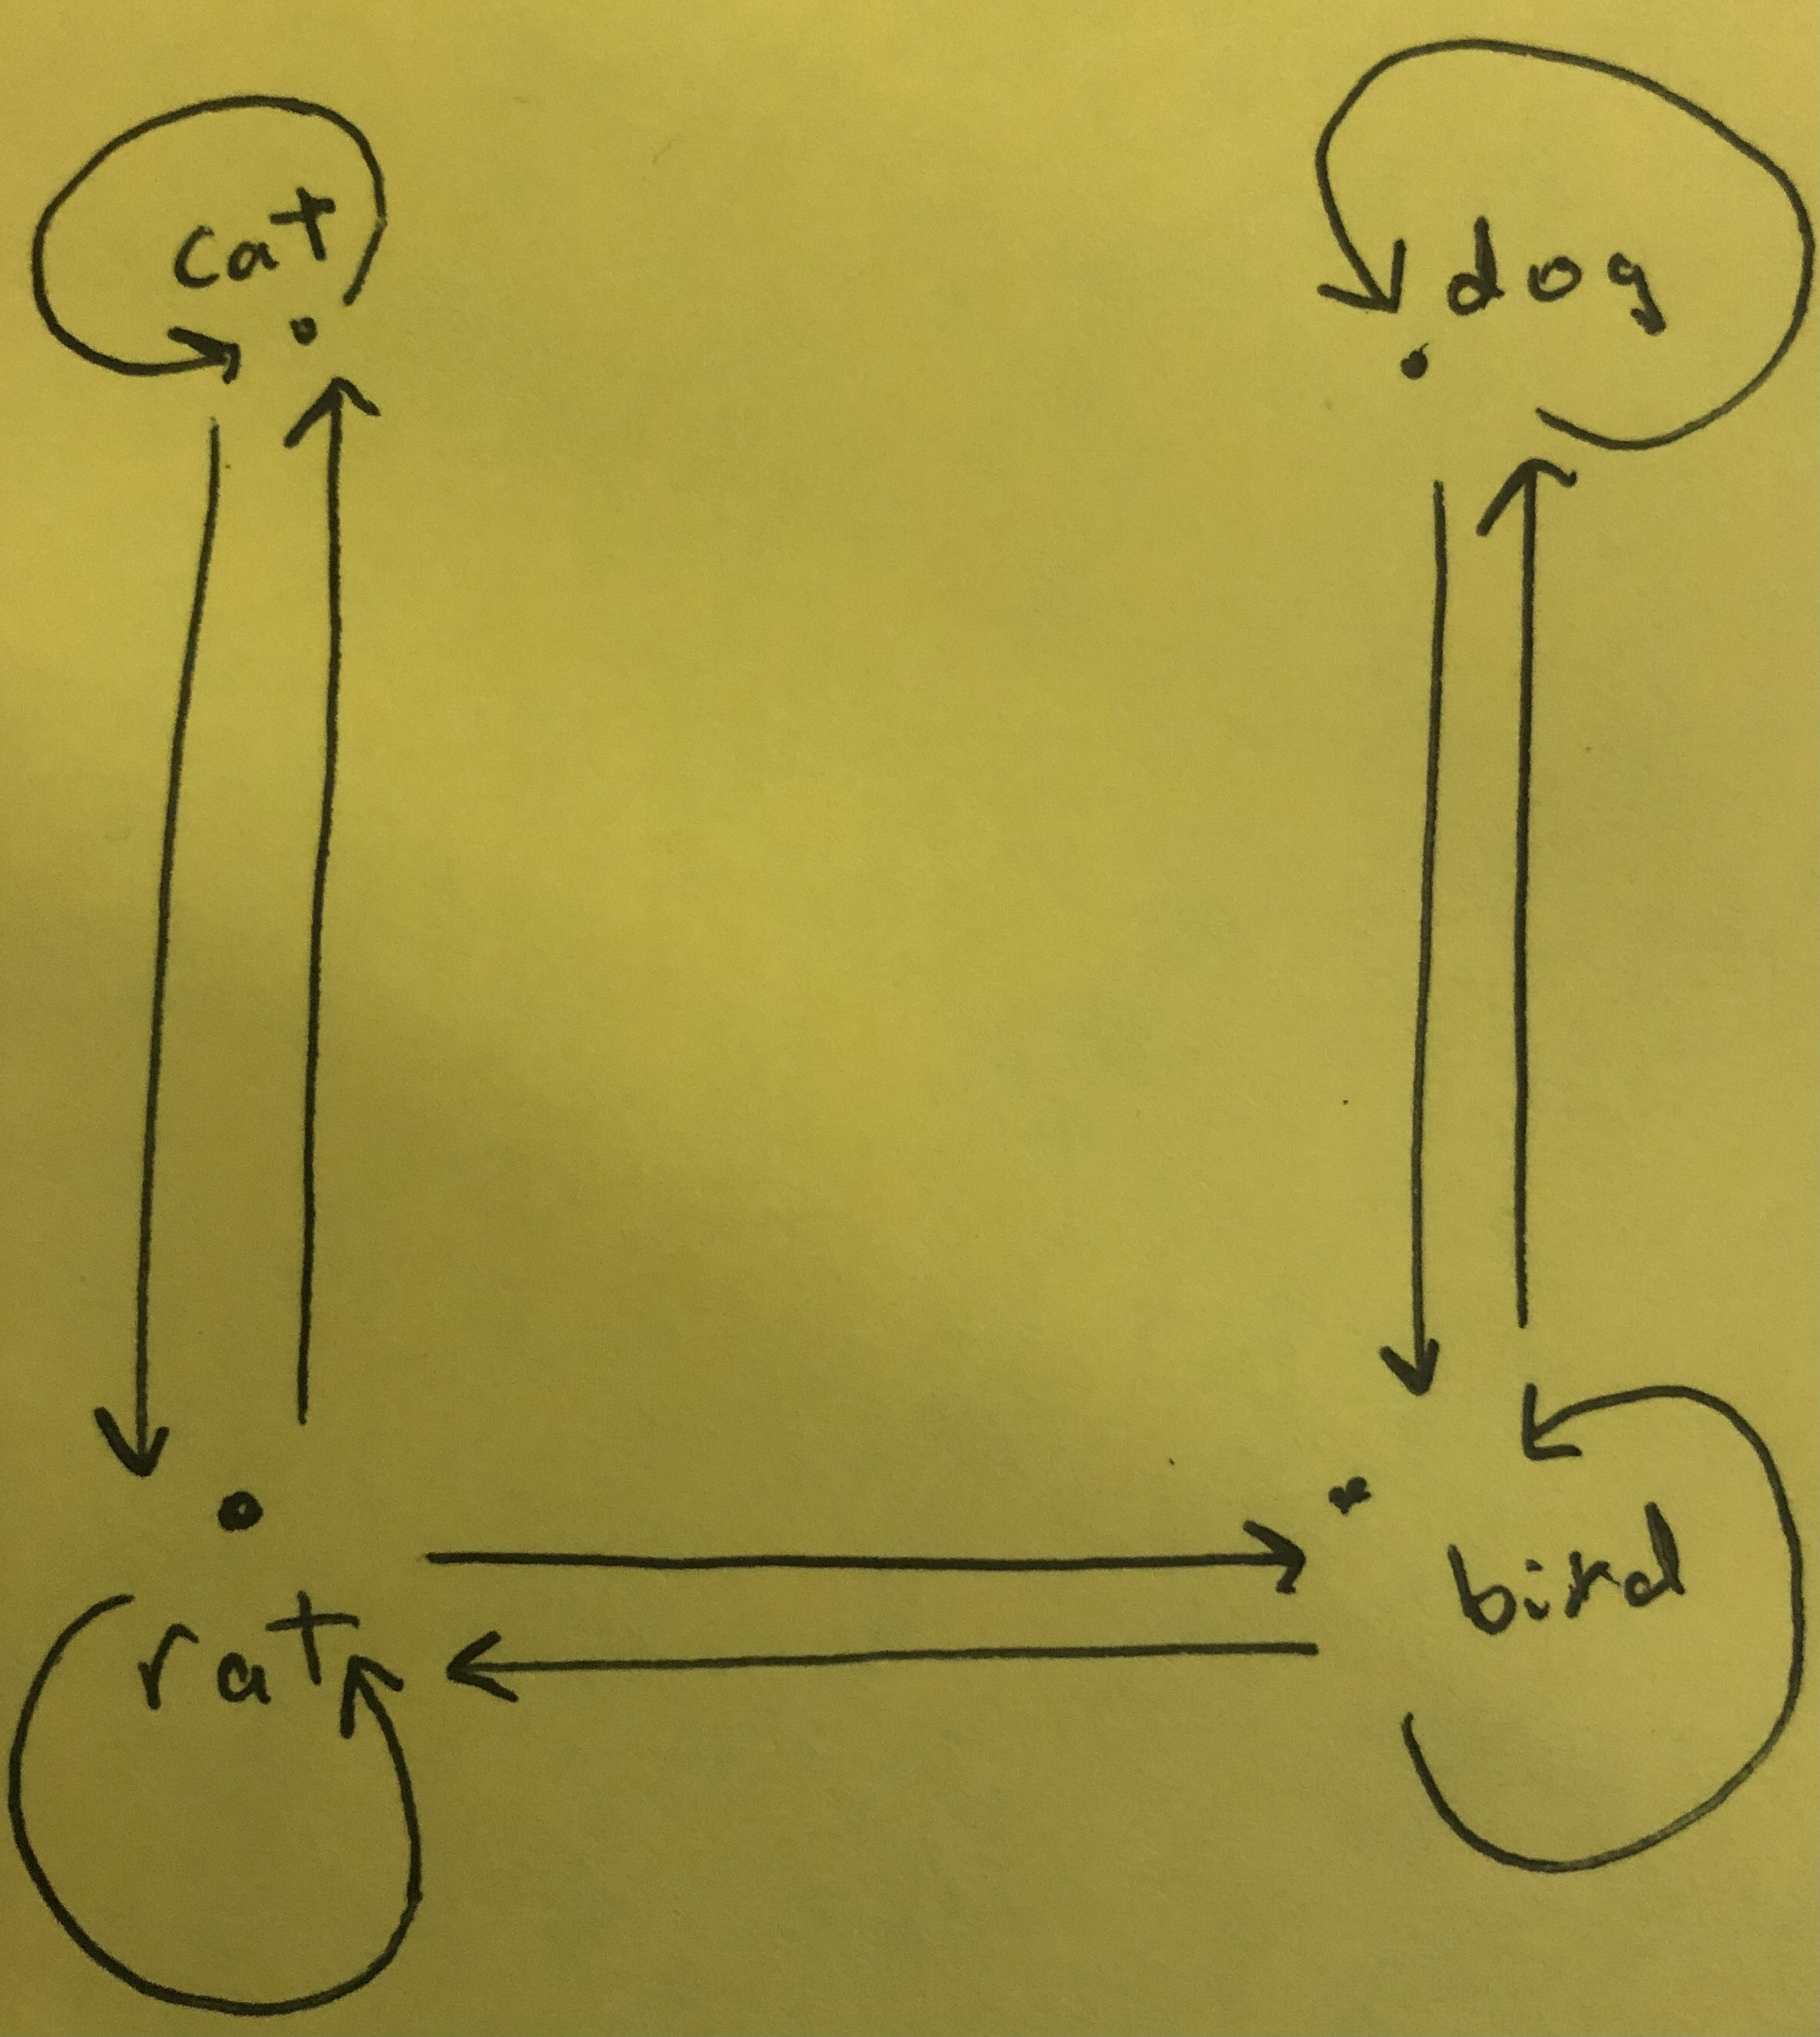
\includegraphics[scale=0.05]{image0.jpg} \\
Minimal expression: $x \bar{z} + \bar{x} z$.

\item Using the Quine-McClusky method, find a minimal expression: \\
$\bar{v} \bar{w} x \bar{y}  \bar{z} + v \bar{w} x \bar{y}  \bar{z} = (v + \bar{v}) \bar{w} x \bar{y}  \bar{z} = (1) \bar{w} x \bar{y}  \bar{z}$\\
$\bar{v} \bar{w} x y  \bar{z} + v \bar{w} x y  \bar{z} = (v + \bar{v}) \bar{w} x y \bar{z} = (1) \bar{w} x y \bar{z}$\\
$\bar{w} x \bar{y} \bar{z} + \bar{w} x y \bar{z} = \bar{w} x (y + \bar{y}) \bar{z} = \bar{w} x \bar{z}$\\
$\bar{v} w x \bar{y} z + v w x \bar{y} z = (v + \bar{v}) w x \bar{y} z = w x \bar{y} z$ \\
Minimal expression: $\bar{w} x \bar{z} + w x \bar{y} z$.

\item Find a regular expression for the language of all binary strings containing an odd number of 1's. \\
Regex: $0^{*} 1 (0^{*} | 1 0^{*} 1)^{*}$

\item Design a deterministic finite automaton that accepts all binary strings that correspond to a value divisible by 3. For example, it should accept 110 (since it is divisible by 3), but not 101 (since 5 is not divisble by 3.)\\
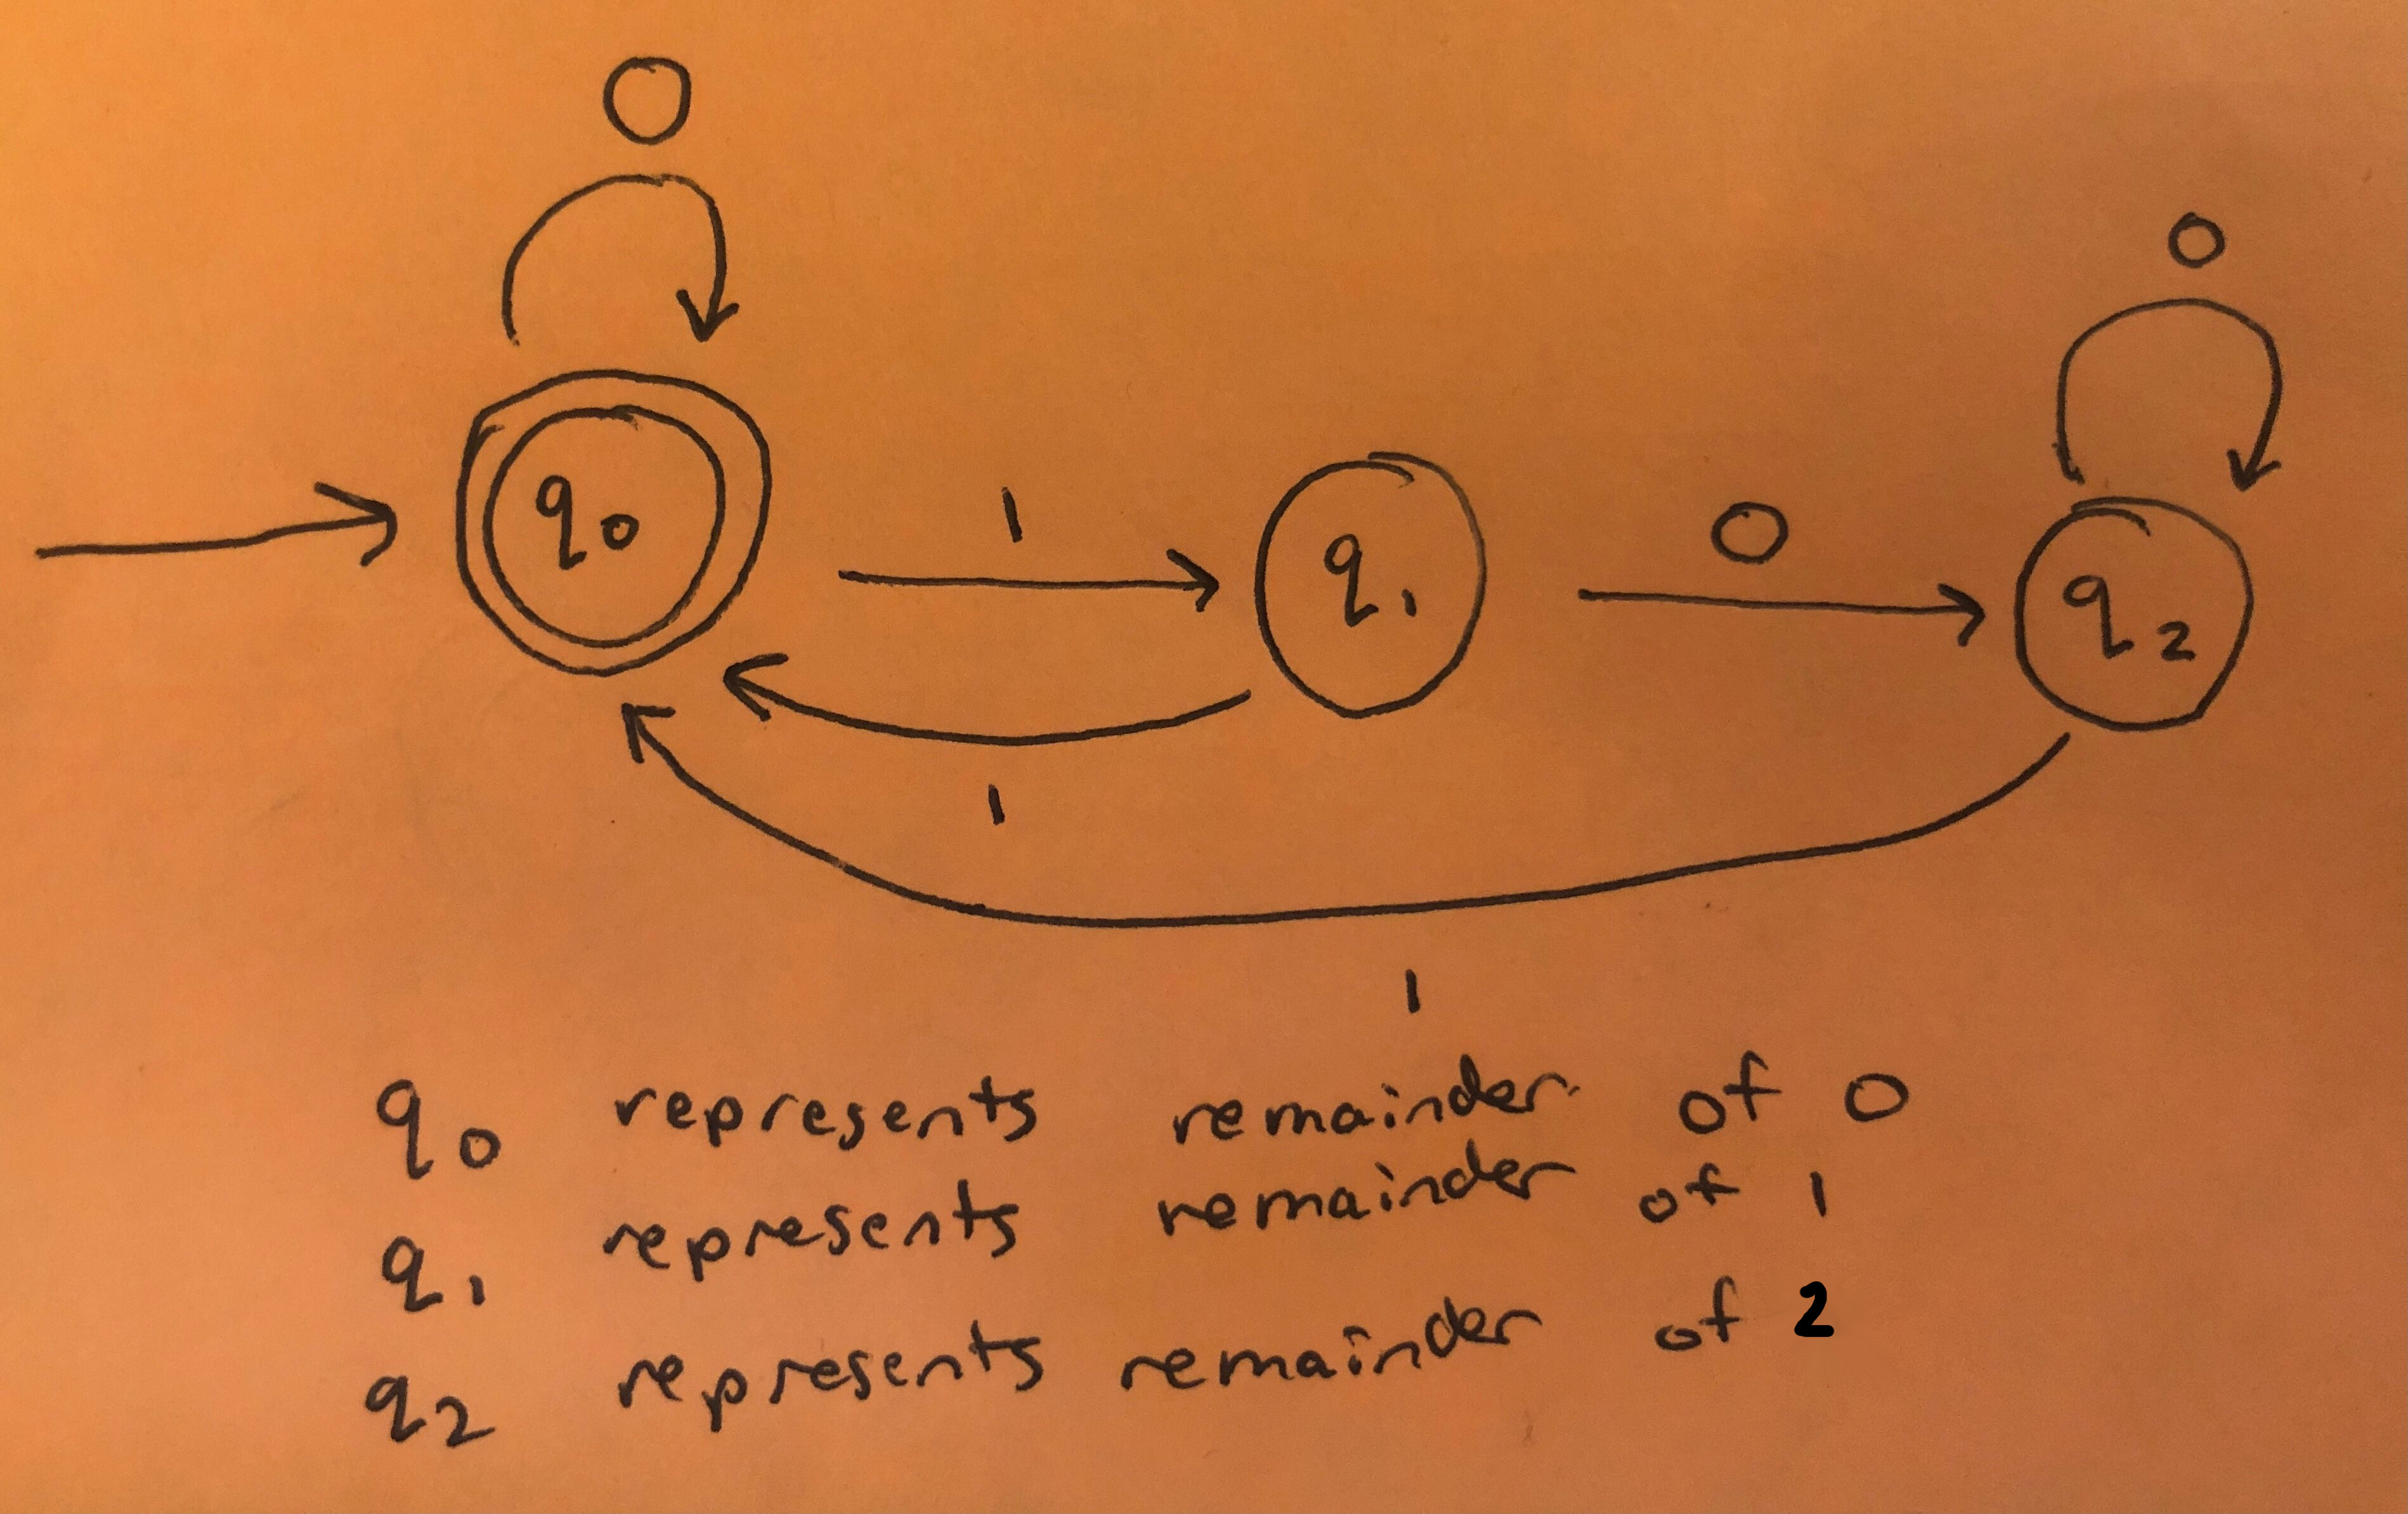
\includegraphics[scale=0.1]{image1.jpg}

\end{enumerate}
\end{document}
